%%%%%%%%%%%%%%%%%%%%%%%%%%%%%%%%%%%%%%%%%
% Formal Text-Rich Title Page 
% LaTeX Template
% Version 1.0 (27/12/12)
%
% This template has been downloaded from:
% http://www.LaTeXTemplates.com
%
% Original author:
% Peter Wilson (herries.press@earthlink.net)
%
% License:
% CC BY-NC-SA 3.0 (http://creativecommons.org/licenses/by-nc-sa/3.0/)
% 
% Instructions for using this template:
% This title page compiles as is. If you wish to include this title page in 
% another document, you will need to copy everything before 
% \begin{document} into the preamble of your document. The title page is
% then included using \titleGP within your document.
%
%%%%%%%%%%%%%%%%%%%%%%%%%%%%%%%%%%%%%%%%%

%----------------------------------------------------------------------------------------
%	PACKAGES AND OTHER DOCUMENT CONFIGURATIONS
%----------------------------------------------------------------------------------------

\documentclass[a4paper]{article}
\usepackage[utf8]{inputenc}
\usepackage[spanish]{babel}
\usepackage{titlesec}
\usepackage{listings}
\usepackage{color}
\usepackage{pdfpages}
\usepackage{verbatim}
\titlelabel{\thetitle.\quad}
\lstset{
  language=C,                % choose the language of the code
  numbers=left,                   % where to put the line-numbers
  stepnumber=1,                   % the step between two line-numbers.        
  numbersep=5pt,                  % how far the line-numbers are from the code
  backgroundcolor=\color{white},  % choose the background color. You must add \usepackage{color}
  showspaces=false,               % show spaces adding particular underscores
  showstringspaces=false,         % underline spaces within strings
  showtabs=false,                 % show tabs within strings adding particular underscores
  tabsize=2,                      % sets default tabsize to 2 spaces
  captionpos=b,                   % sets the caption-position to bottom
  breaklines=true,                % sets automatic line breaking
  breakatwhitespace=true,         % sets if automatic breaks should only happen at whitespace
  title=\lstname,                 % show the filename of files included with \lstinputlisting;
}


%----------------------------------------------------------------------------------------
%	TITLE PAGE
%----------------------------------------------------------------------------------------

\newcommand*{\titleGP}{\begingroup % Create the command for including the title page in the document
\centering % Center all text
\vspace*{\baselineskip} % White space at the top of the page

\rule{\textwidth}{1.6pt}\vspace*{-\baselineskip}\vspace*{2pt} % Thick horizontal line
\rule{\textwidth}{0.4pt}\\[\baselineskip] % Thin horizontal line

{\LARGE \textbf{ORGANIZACIÓN DE COMPUTADORAS}\\[1\baselineskip]INFORME\\[0.2\baselineskip] TRABAJO PRÁCTICO 0}\\[0.2\baselineskip] % Title

\rule{\textwidth}{0.4pt}\vspace*{-\baselineskip}\vspace{3.2pt} % Thin horizontal line
\rule{\textwidth}{1.6pt}\\[\baselineskip] % Thick horizontal line

\vspace*{2\baselineskip} % Whitespace

\textbf{Alumnos} \\[\baselineskip]
{ 93198 - Peña, Maximiliano \\ maxipenia@gmail.com  \\[1\baselineskip]

 93665 - Poggio, Demian \\ demianpoggio@gmail.com  \\[1\baselineskip] 
 
 95505 - Iogha, Octavio \\ octaviomdq93@gmail.com \par} % Editor list

\vspace*{4\baselineskip} % Whitespace
	
% \textbf{Fecha de Entrega} \\[\baselineskip]
% { Martes 29 de Marzo }

\vspace*{4\baselineskip} % Whitespace

\textbf{Fecha de Vencimiento} \\[\baselineskip]
{ Martes 1 de Noviembre }

\endgroup}

%----------------------------------------------------------------------------------------
%	BLANK DOCUMENT
%----------------------------------------------------------------------------------------

\begin{document} 

\pagestyle{empty} % Removes page numbers

\titleGP % This command includes the title page

\newpage

\pagestyle{plain}

\section{Objetivos}
	El objetivo de este trabajo práctico es adaptar una función implementada en lenguaje C, al lenguaje Assembly MIPS32. Para ello, se volvieron a utilizar las herramientas ya vistas en el TP0.

\section{Introducción Teórica}
  \label{sec:InfoTeo}
 A partir de una imágen patrón del programa encargado de dibujar las regiones de Julia, se debe analizar el funcionamiento del algoritmo, e implementarlo correctamente en el lenguaje Assembly MIPS.\\
 En la implementación del mismo, además del uso de las funciones provistas por el lenguaje assembler, también se han tenido que hacer uso de las syscalls, específicamente la llamada al sistema \texttt{"SYS{\_}WRITE"}.

		

\subsection{Compilación}
NOTA: Dependiendo de qué archivo se quiera utilizar para compilar la imágen, el Makefile.in puede contener modificaciones en la línea 6.\\
Suponiendo que se quiere utilizar la versión implementada en MIPS assembly, entonces la línea 6 debe ser:\\
\texttt{SRCS = mips32{\_}plot.S main.c mygetopt{\_}long.c}.\\
Para compilar el programa,basta con ejecutar 

\bigskip	
\begin{verbatim} 
	make clean
	make makefiles
	make
\end{verbatim}


\section{Corridas de prueba}

\subsection{Pruebas}
Se corre con las opciones por defecto de la imágen patrón, y se obtiene:
\bigskip

\includegraphics[width=0.8\textwidth,natwidth=610,natheight=642]{imgs/output.png}

\bigskip
Lo cual coincide con la imágen esperada.

\bigskip
\bigskip
Ahora se corre con el centro corrido, precisamente: \\
\texttt{./tp1 -c 0.282+0.01i}\\

\includegraphics[width=0.8\textwidth,natwidth=610,natheight=642]{imgs/output2.png}

\bigskip

Lo cual coincide con la imágen esperada.\\

Por último, se corre la siguiente línea:\\
\texttt{\$  ./tp1 -C -1.125-0.21650635094611i}\\

\includegraphics[width=0.8\textwidth,natwidth=610,natheight=642]{imgs/output3.png}

\bigskip

Nuevamente se obtiene el resultado esperado.

\section{Código MIPS}


\bigskip

\lstinputlisting{mips32_plot.S}

\section{Conclusión}
	En este trabajo práctico, se han podido utilizar todas las herramientas inicialmente presentadas en el TP0, aplicandolas a la implementación de una función hecha en C, en lenguaje assembler MIPS32.\\
	Por otro lado, se ha podido practicar el uso de la ABI dada por la cátedra, para el desarrollo de las diferentes funciones implementadas en el lenguaje assembly.\\
	Por último, se ha podido interactuar con el sistema operativo netBSD, al hacer uso de las llamadas al sistema, o "syscalls", para escribir un buffer de tamaño predeterminado al archivo resultante.

\section{Enunciado}

Adjundto a partir de la siguiente hoja.

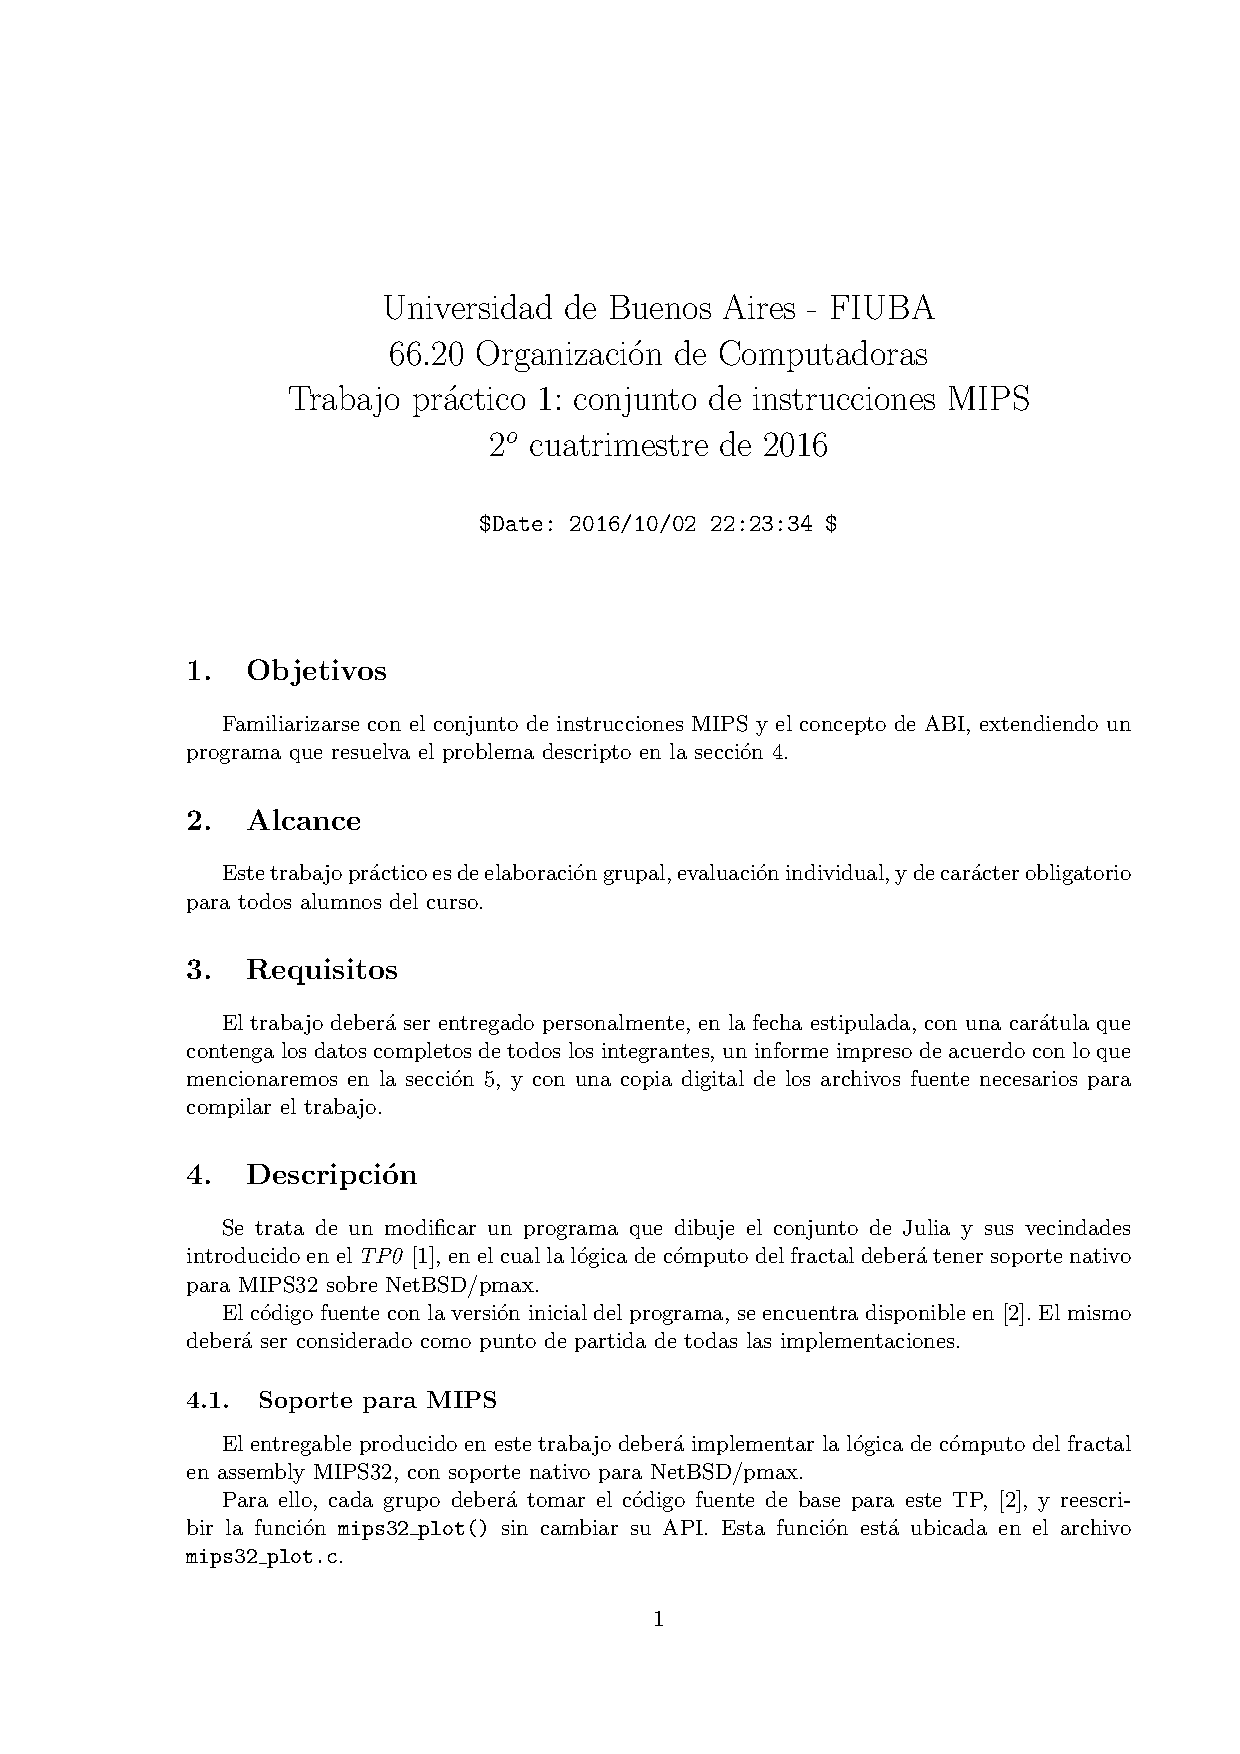
\includepdf[pages={-}]{enunciadotp1.pdf}

\end{document}
